
\subsection{Answers}
\begin{table}[htb]%
\begin{center}%
\caption{Q17: What aspects of the MPI standard do you use in your program in its current form?}%
\label{tab:Q17-ans}%
\begin{tabular}{l|l|r}%
\hline%
Choice & Abbrv. & \# Answers \\%
\hline%
Collective communications & Collectives & 740 (89.0\%) \\%
Point-to-point communications & Point-to-pint & 710 (85.4\%) \\%
MPI datatypes & Datatypes & 521 (62.7\%) \\%
MPI with OpenMP (or multithread) & with OpenMP & 478 (57.5\%) \\%
{\small Communicator operations (split, duplicat$\cdots$} & Communicator & 412 (49.6\%) \\%
One-sided communications & One-sided & 226 (27.2\%) \\%
PMPI interface & PMPI & 67 (8.1\%) \\%
Persistent communications & Persistent & 61 (7.3\%) \\%
Dynamic process creation & Dyn. process & 51 (6.1\%) \\%
other & - & 20 (2.4\%) \\%
\hline%
\multicolumn{2}{c}{total} & 3286 (831)\\%
\hline%
\end{tabular}%
\end{center}%
\end{table}%


\subsection{List of other answers}
\begin{itemize}
\item Europe:France: I use almost exclusively the Boost MPI layer
\item Europe:France: MPI/IO
\item Europe:France: communications progression
\item Europe:Germany: MPI I/O
\item Europe:Germany: MPI I/O
\item Europe:Germany: MPI-IO
\item Europe:Germany: MPI-IO, plan to use shared memory window for hybrid parallelization
\item Europe:Germany: None
\item Europe:Italy: MPI-IO
\item Europe:UK: MPI-I/O, Shared Memory
\item Europe:UK: MPI-IO, non-blocking collectives
\item Europe:others: CUDA-aware MPI
\item Europe:others: Cartesian topologies
\item Europe:others: I have no idea
\item Europe:others: MPI + CUDA C / CUDA-aware MPI
\item Europe:others: cuda-aware mpi (although I think that is not standard is it?)
\item Europe:others: no programs
\item Japan: I don't know so well.
\item Russia: MPI I/O
\item Russia: no one

\end{itemize}

\begin{figure}[htb]
\begin{center}
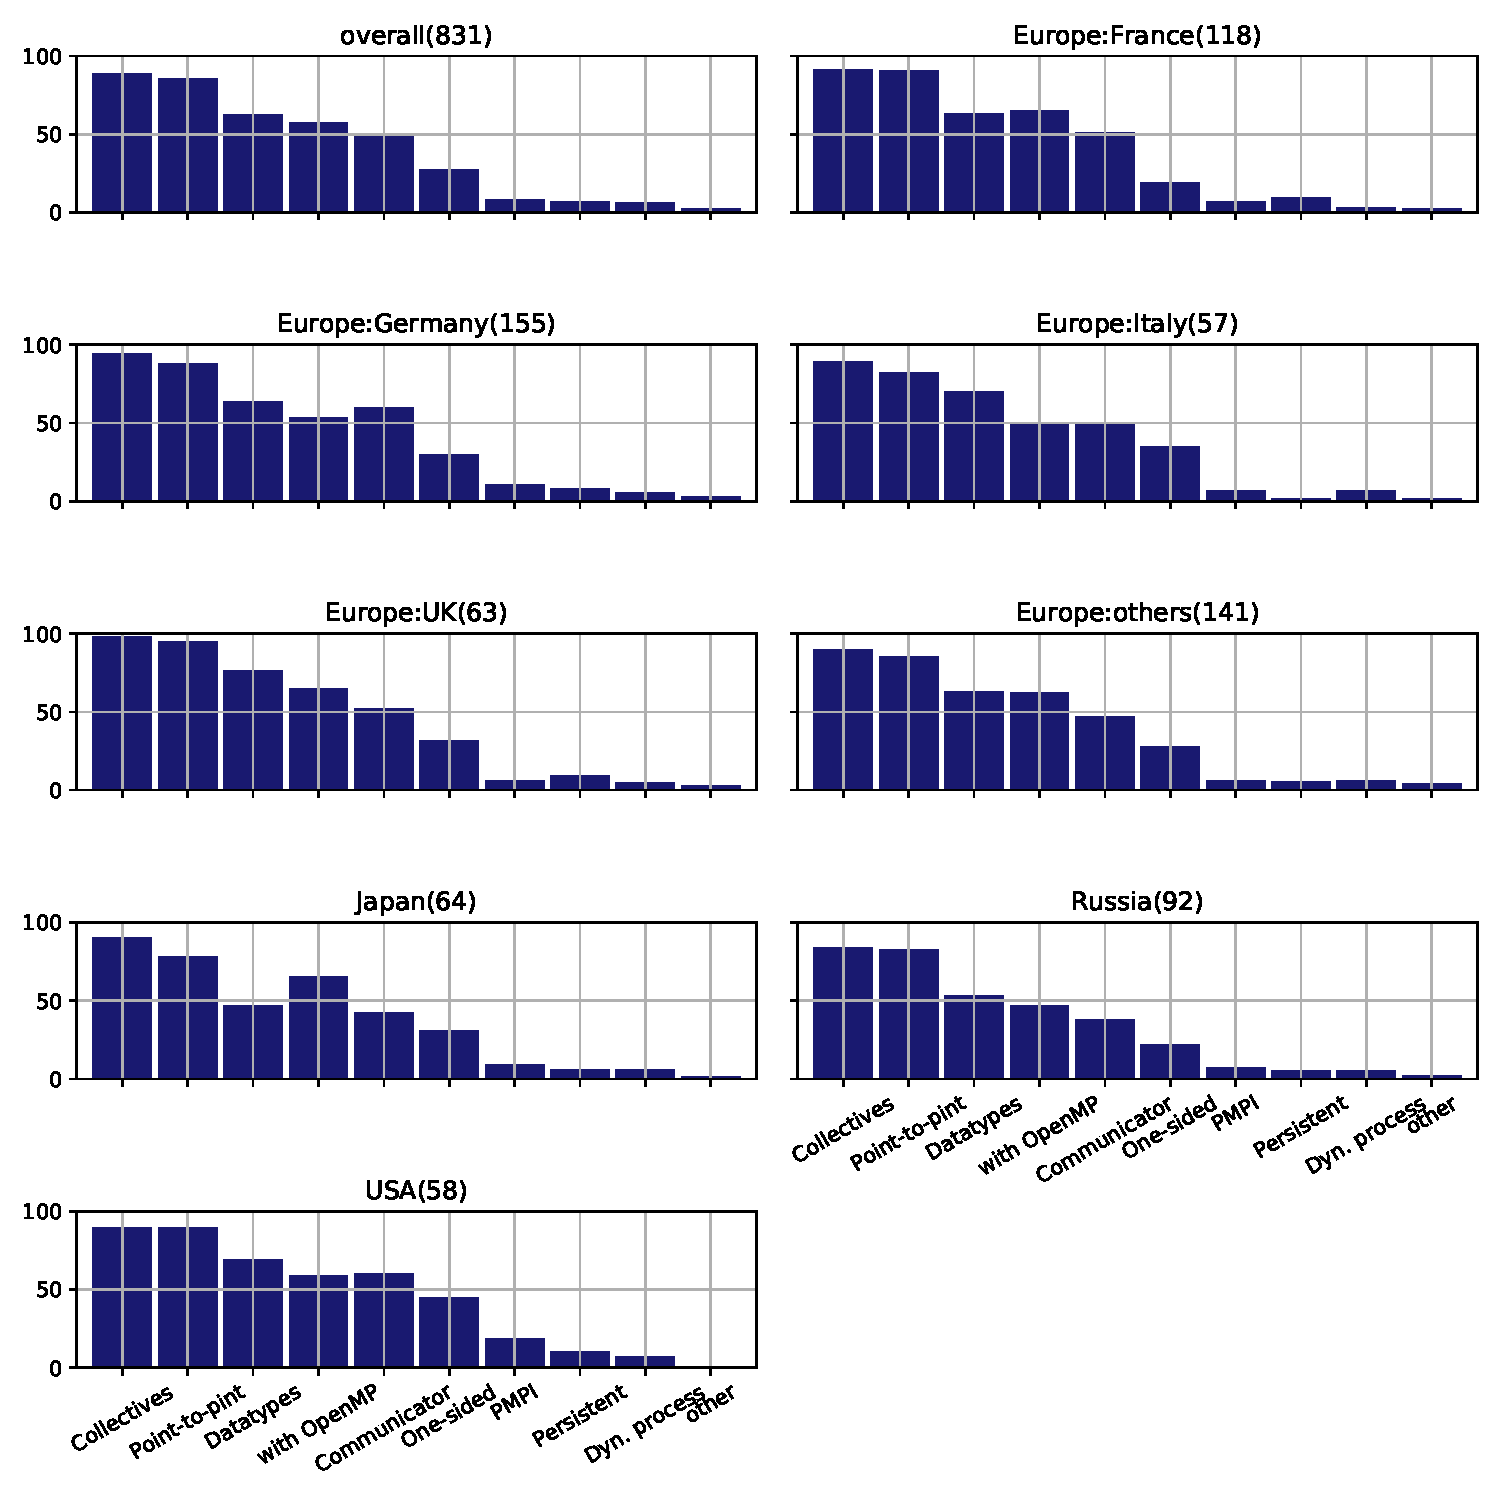
\includegraphics[width=10cm]{../pdfs/Q17.pdf}
\caption{Simple analysis: Q17}
\label{fig:Q17}
\end{center}
\end{figure}

The answers given here are not really surprising. We see that the most used
features are the one that are very close the MPI programming model
(communication, and data type management) with 60\% of the answers. We also see
that the forth most useful feature concerns MPI+thread (OpenMP or Pthread),
meaning that programming multicore system is often done by mixing different
programming models.  

Related to the previous question, we see that the most used features are also
among the most known one and that the three less used features (PMPI, persistent
communication, dynamic process creation) are also the less known ones. 
